\section{Drehencoder}
Um Eingaben vom Benutzer, wie zum Beispiel lauter/leiser, Radiostation wechseln und so weiter, anzunehmen, haben wir einen Drehencoder an das Radio angeschlossen.
\newline
Der Unterschied von einem Drehencoder zu einem normalen Potentiometer ist der, das er sich endlos drehen lässt und digital seine Drehrichtung ausgibt.
\newline
Er besteht im inneren aus zwei Tastern, die sich je nach Drehrichtung öffnen und schließen. Der Zustand der zwei Taster muss ausgelesen und als Zustand gespeichert werden. Aus der Abfolge dieses entstehenden Binärcodes kann man dann die Drehrichtung bestimmen.

\begin{figure}[H] 
  \centering
     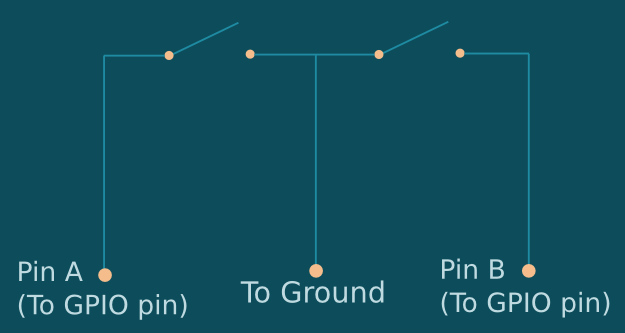
\includegraphics[width=0.7\textwidth]{Bilder/rotary1.png}
  \caption{Drehencoder-Schema}
  \label{fig:Schema}
\end{figure}

Außerdem verfügt der Drehencoder über einen zusätzlichen Taster, um Eingaben zu bestätigen.


\subsection{Hardware}
Der Drehencoder wird an die GPIO-Pins des Raspberry angeschlossen. Dabei hielten wir uns an folgendes Schema:

\begin{figure}[H] 
  \centering
     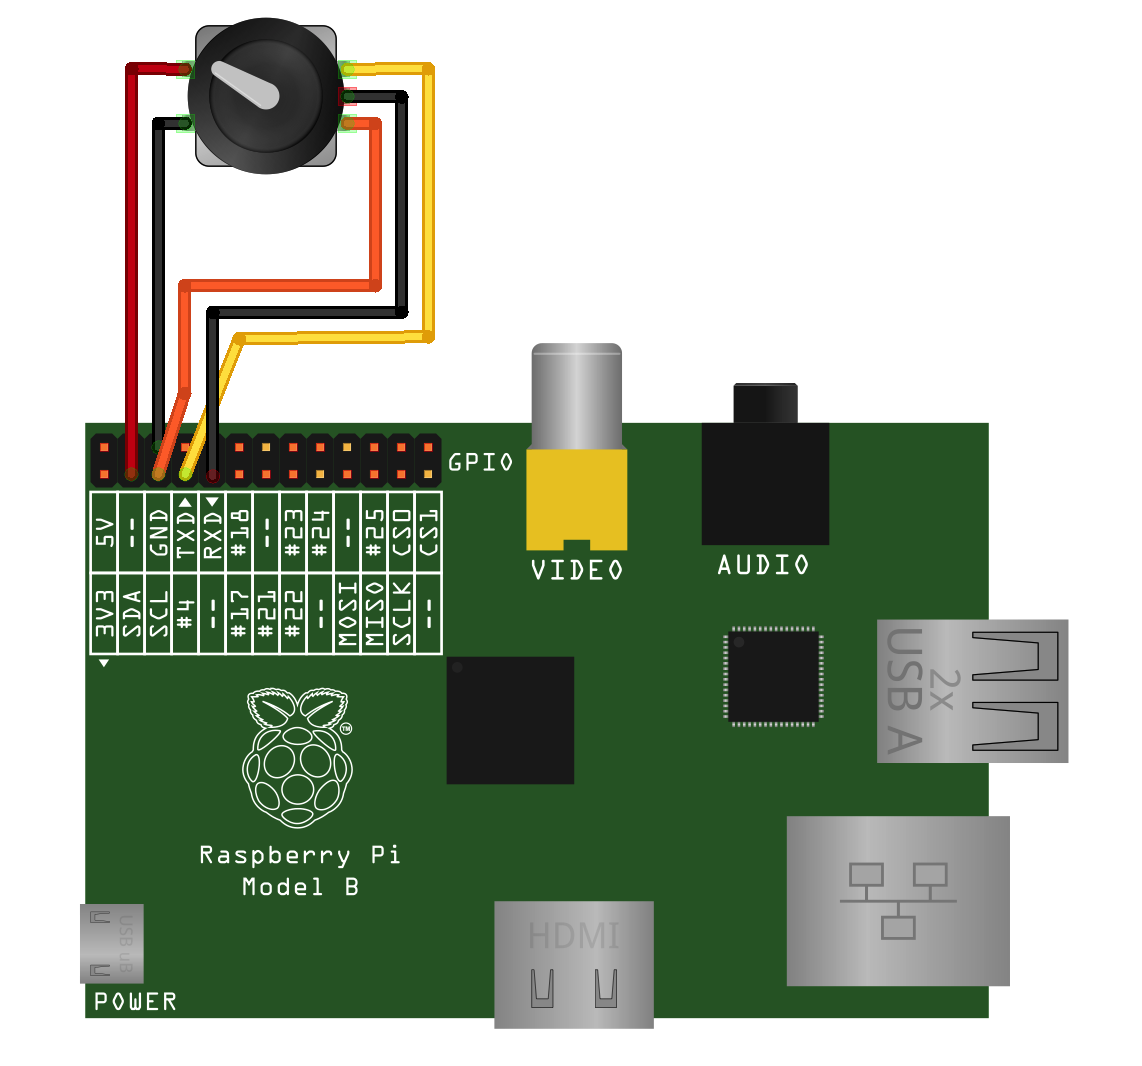
\includegraphics[width=0.7\textwidth]{Bilder/rotary2.png}
  \caption{Drehencoder-Schaltung}
  \label{fig:Schaltung}
\end{figure}

Die beiden Kontakte links vom Drehencoder sind vom Taster. Wird er gedrückt, zieht er den Eingangspin des Raspberrys auf GND. Intern hat der Eingang einen Pull-Up Widerstand eingebaut, sodass das Drücken auf den Taster zuverlässig erkannt werden kann.
Auf der Rechten Seite sind die drei Kontakte des Drehencoders abgebildet. Auch sie sind mit GPIO-Pins bzw. GND verbunden und verfügen über interne Pull-Up Widerstände.

\subsection{Software}
Als erstes wurde eine Encoder-Struct definiert, die intern die Richtung und ob der Knopf gedrückt wurde speichert. Außerdem werden hier die Pin-Nummern angegeben, an die der Encoder angeschlossen ist.
\begin{lstlisting}[label=struct_encoder,caption=Encoder Struct]
struct encoder
{
    int pin_a;
    int pin_b;
	 int  pin_button;
	volatile int button_pressed;
   volatile int lastEncoded;
	volatile direction direction;
};
\end{lstlisting}

Um die Zustände des Drehencoders auszulesen wurde die wiringPi Bibliothek genutzt. 
\newline
Dabei werden die Eingangspins als Interrupts definiert, damit wiringPi sich automatisch um die Abfrage kümmert und eine Interrupt Service Routine aufruft, wenn eine Signaländerung erkannt wurde.

\begin{lstlisting}[label=encoder_init,caption=Encoder Initialiserung]
pinMode(pin_a, INPUT);
pinMode(pin_b, INPUT);
pinMode(pin_button, INPUT);
pullUpDnControl(pin_a, PUD_UP);
pullUpDnControl(pin_b, PUD_UP);
wiringPiISR(pin_a,INT_EDGE_BOTH, updateEncoders);
wiringPiISR(pin_b,INT_EDGE_BOTH, updateEncoders);
wiringPiISR(pin_button, INT_EDGE_FALLING, updateButton);
\end{lstlisting}

Die beiden Interrupt Service Routinen updateEncoders() und updateButton() werden im nächsten Abschnitt erläutert.

\subsubsection{updateEcoders()}
In der updateEncoders() Funktion wird die Drehrichtung des Encoders ermittelt.
\begin{lstlisting}[label=encoder_update,caption=updateEncoders()]
void updateEncoders()
{
	struct encoder* encoder = &default_encoder;
        int MSB = digitalRead(encoder->pin_a);
        int LSB = digitalRead(encoder->pin_b);

        int encoded = (MSB << 1) | LSB;
        int sum = (encoder->lastEncoded << 2) | encoded;

		encoder->lastEncoded = encoded;
        if(sum == 0b1101 || sum == 0b0100 || 
        	sum == 0b0010 || sum == 0b1011) 
        		encoder->direction=DIR_RIGHT;
        if(sum == 0b1110 || sum == 0b0111 || 
        	sum == 0b0001 || sum == 0b1000) 
        		encoder->direction=DIR_LEFT;
}
\end{lstlisting}
Dazu werden zuerst die aktuellen Zustände der Schalter eingelesen und verkettet in der Variablen "`encoded"' gespeichert. Dann wird "`encoded"' mit dem vorherigen Zustand verkettet und in "`sum"' gespeichert.

Aus diesem Bitmuster lässt sich nun die Drehrichtung ablesen. Bei 1101, 0100, 0010 oder 1011 dreht sich der Encoder nach rechts.
Bei 1110, 0111, 0001 oder 1000 dreht er sich nach links.

Der aktuelle Zustand wird dann noch als "`lastEncodes"' abgespeichert und die Funktion ist beendet.
\newline
Mit der Funktion getDirection(struct encoder *encoder) kann dann vom Hauptprogramm die Richtung abgefragt werden.

\subsubsection{updateButton()}
In der updateButton() Funktion wird der Druck auf den Knopf in der encoder struct abgespeichert, und kann dann vom Hauptprogramm mit getButtonPressed(struct encoder *encoder) abgefragt werden.

\begin{lstlisting}[label=encoder_buttonr,caption=updateButton()]
void updateButton()
{
	default_encoder.button_pressed=1;
}
\end{lstlisting}
Der GPIO-Pin muss hier nicht extra abgefragt werden, da der Interrupt nur aufgerufen wird, falls der Knopf gedrückt wurde.